\section{ Definite Integrals}
%\int^{b}_{a}

\textbf{Property I : First Fundamental Theorem of Calculus}

\vspace{5mm}
Let $f$ be a continuous function on an interval $[a,b]$ and $A(x)$ be the area function.

\vspace{2mm}

\begin{tcolorbox}
\begin{center}
\[ \text{Area Function A(x)} = \int_{a}^{b} f(x).dx \]
\end{center}
\end{tcolorbox}

\begin{figure}[ht]
    \centering
    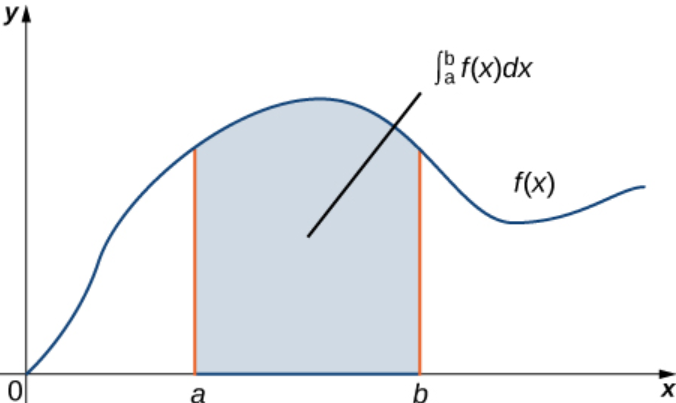
\includegraphics[scale=1]{definite_integrals} 
    \label{definite_int}
\end{figure}


\textbf{Property II : Second Fundamental Theorem of Calculus}

\vspace{5mm}

\begin{tcolorbox}
\begin{center}
\[\int_{a}^{b} f(x).dx = [F(x)]^{b}_{a} = F(a) - F(b) \]
\end{center}
\end{tcolorbox}

\vspace{5mm}

\begin{align}
&\int^{b}_{a} f(x).dx = - \int^{a}_{b} f(x).dx \\[5mm]
&\int^{b}_{a} f(x).dx = \int^{c}_{a} f(x).dx + \int^{b}_{c} f(x).dx \quad \text{where} \: a<c<b \\[5mm]
&\int^{a}_{0}f(x).dx = \int^{a}_{0}f(a-x).dx
\end{align}

\begin{align}
&\int^{a}_{-a}f(x).dx = 
\begin{cases}
2.\int^{a}_{0} f(x).dx \quad \text{if} \: f(x) = f(-x) \\
0 \quad if \: f(x) = -f(-x) \\
\end{cases}
\\[5mm]
&\int^{2a}_{0}f(x).dx = 
\begin{cases}
2.\int^{a}_{0}f(x).dx \quad if \: f(2a-x) = f(x) \\
0 \quad if \: f(2a-x) = -f(x) \\
\end{cases}
\end{align}

\vspace{5mm}

Mean value of a function in an interval $(a,b)$ is given by:

\begin{tcolorbox}
\begin{center}
\[ \frac{1}{b-a} \int_{a}^{b} f(x).dx \]
\end{center}
\end{tcolorbox}